\section{Quantità di vegetazione in alveo}
Si è quantificato l'areale delle isole presenti in alveo avendo accortezza di distinguerlo chiaramente dall'areale della \emph{floodplain}, il quale è soggetto a dinamiche diverse rispetto alle isole.

\subsection{Metodi: classificare l'alveo}
Per classificare il terreno occupato dall'alveo è stato seguito l'approccio di altri autori in analisi simili eseguite su immagini \AST{} e LandSat~TM \squarecites{Bertoldi:2011-ASTER}{Henshaw:2013-LandSat}.
%
\begin{description}
	\item[Maschera computazionale] 
	Dapprima è stata individuata manualmente una maschera di calcolo che comprendesse l'alveo attivo e la parte di piana alluvionale che è stata erosa quando coinvolta nelle piene; 
	tale maschera si estende da Tolmezzo al ponte di Madrisio
	(\vref{fig:esempio-maschera}). 
	Applicandola, il dominio computazionale è stato ridotto a comprendere l'inviluppo degli alvei attivi che si sono succeduti dall'immagine del~2000 a quella del~2018.
	%
	\begin{figure}[t]
		\centering
		\begin{subfigure}[b]{0.4\textwidth}
			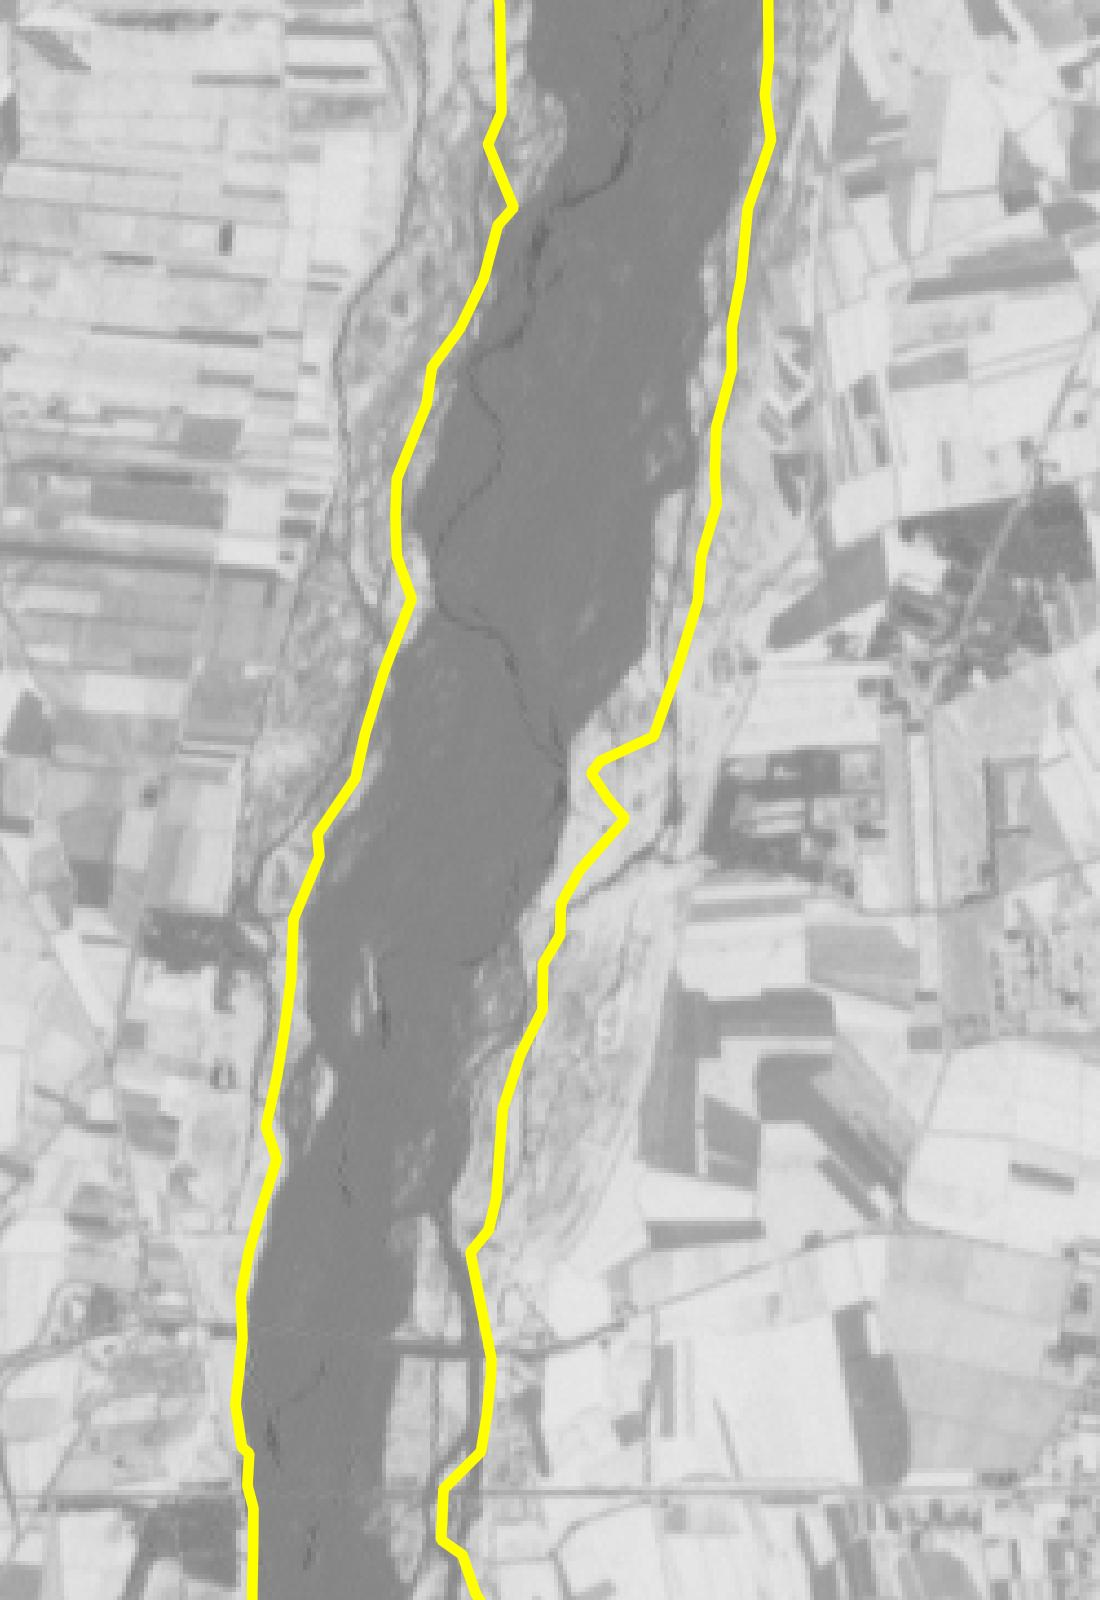
\includegraphics[width=\textwidth]{files/esempio_mask_2002_06_12.jpeg}
			\caption{\AST{} 2002-06-12.}
		\end{subfigure}
		\qquad
		\begin{subfigure}[b]{0.4\textwidth}
			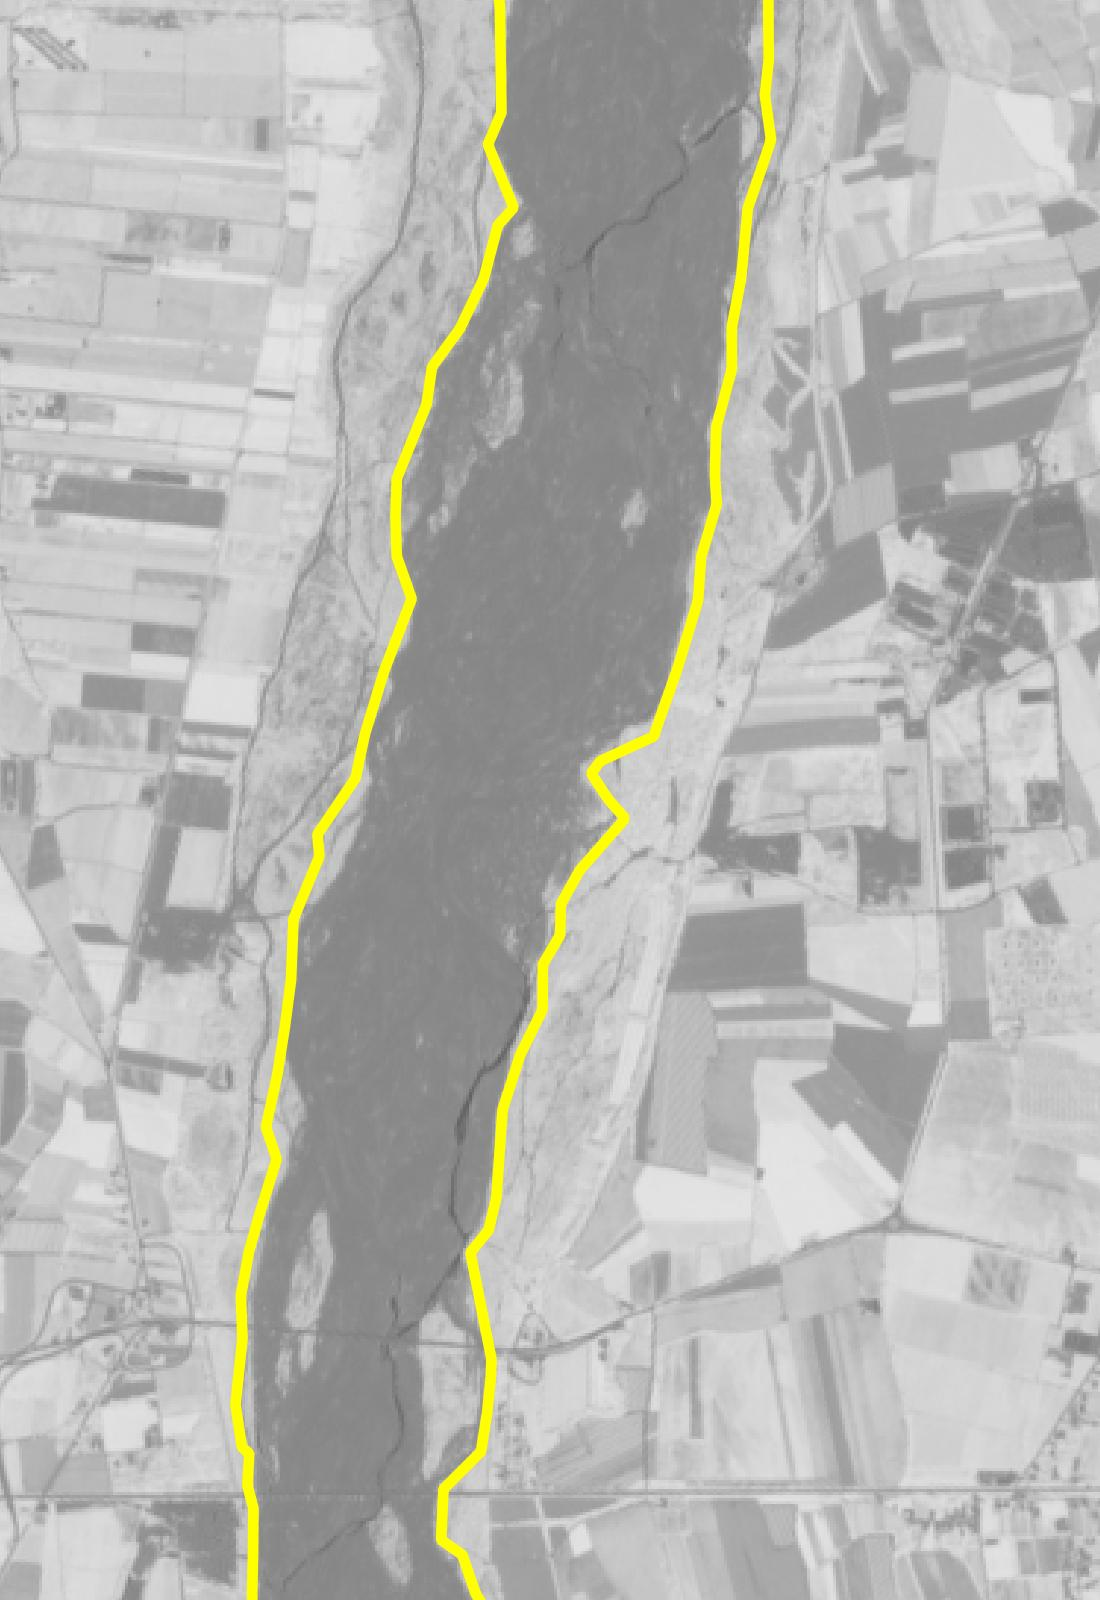
\includegraphics[width=\textwidth]{files/esempio_mask_2015_09_12.jpeg}
			\caption{\Se{} 2015-09-12.}
		\end{subfigure}
		\caption[definizione della maschera per limitare il dominio computazionale]
			{esempio in cui si vede come la maschera utilizzata per limitare il dominio computazionale (in giallo) sia il risultato dell'inviluppo degli alvei attivi che si sono modificati nel tempo; le immagini sono le mappe di NDVI.}
		\label{fig:esempio-maschera}
	\end{figure}
	%
	%
	\item[NDVI] 
	In questa area è stato calcolato il \emph{Normalized Difference Vegetation Index} (NDVI) grazie alle bande del \emph{Near Infrared} (NIR) e del \emph{Red} (R)
	%
	\begin{equation}
		%\notag
		NDVI = \frac{NIR - R}{NIR + R} \quad .
		\label{eq:ndvi}
	\end{equation}
	%
	%
	\item[Aree campione]
	\`{E} stata effettuata una digitalizzazione manuale di alcune aree campione per le immagini \AST{} del~2005-08-30 ($\sim 70$) e del~2012-08-01 ($\sim 100$), le immagini Plaiades del~2014-10-31 ($\sim 40$) e del~2015-06-13 ($\sim 40$), l'immagine \Se{} del~2017-04-21 ($\sim 45$) e l'immagine \WV{} del 2018-06-15 ($\sim 55$) (\vref{fig:esempio-aree-campione}).
	Sono state selezionate immagini per ogni satellite poiché ciascuno è sensibile a bande leggermente diverse. 
	%; si sono osservate due immagini \AST{} dato il grande numero di immagini disponibili da questo sensore scegliendo quelle con minor nuvolosità.
	\\
	Queste aree campione sono state suddivise in tre classi: vegetazione, alveo attivo e canale.
	%
	\begin{figure}[ht]
		\centering
		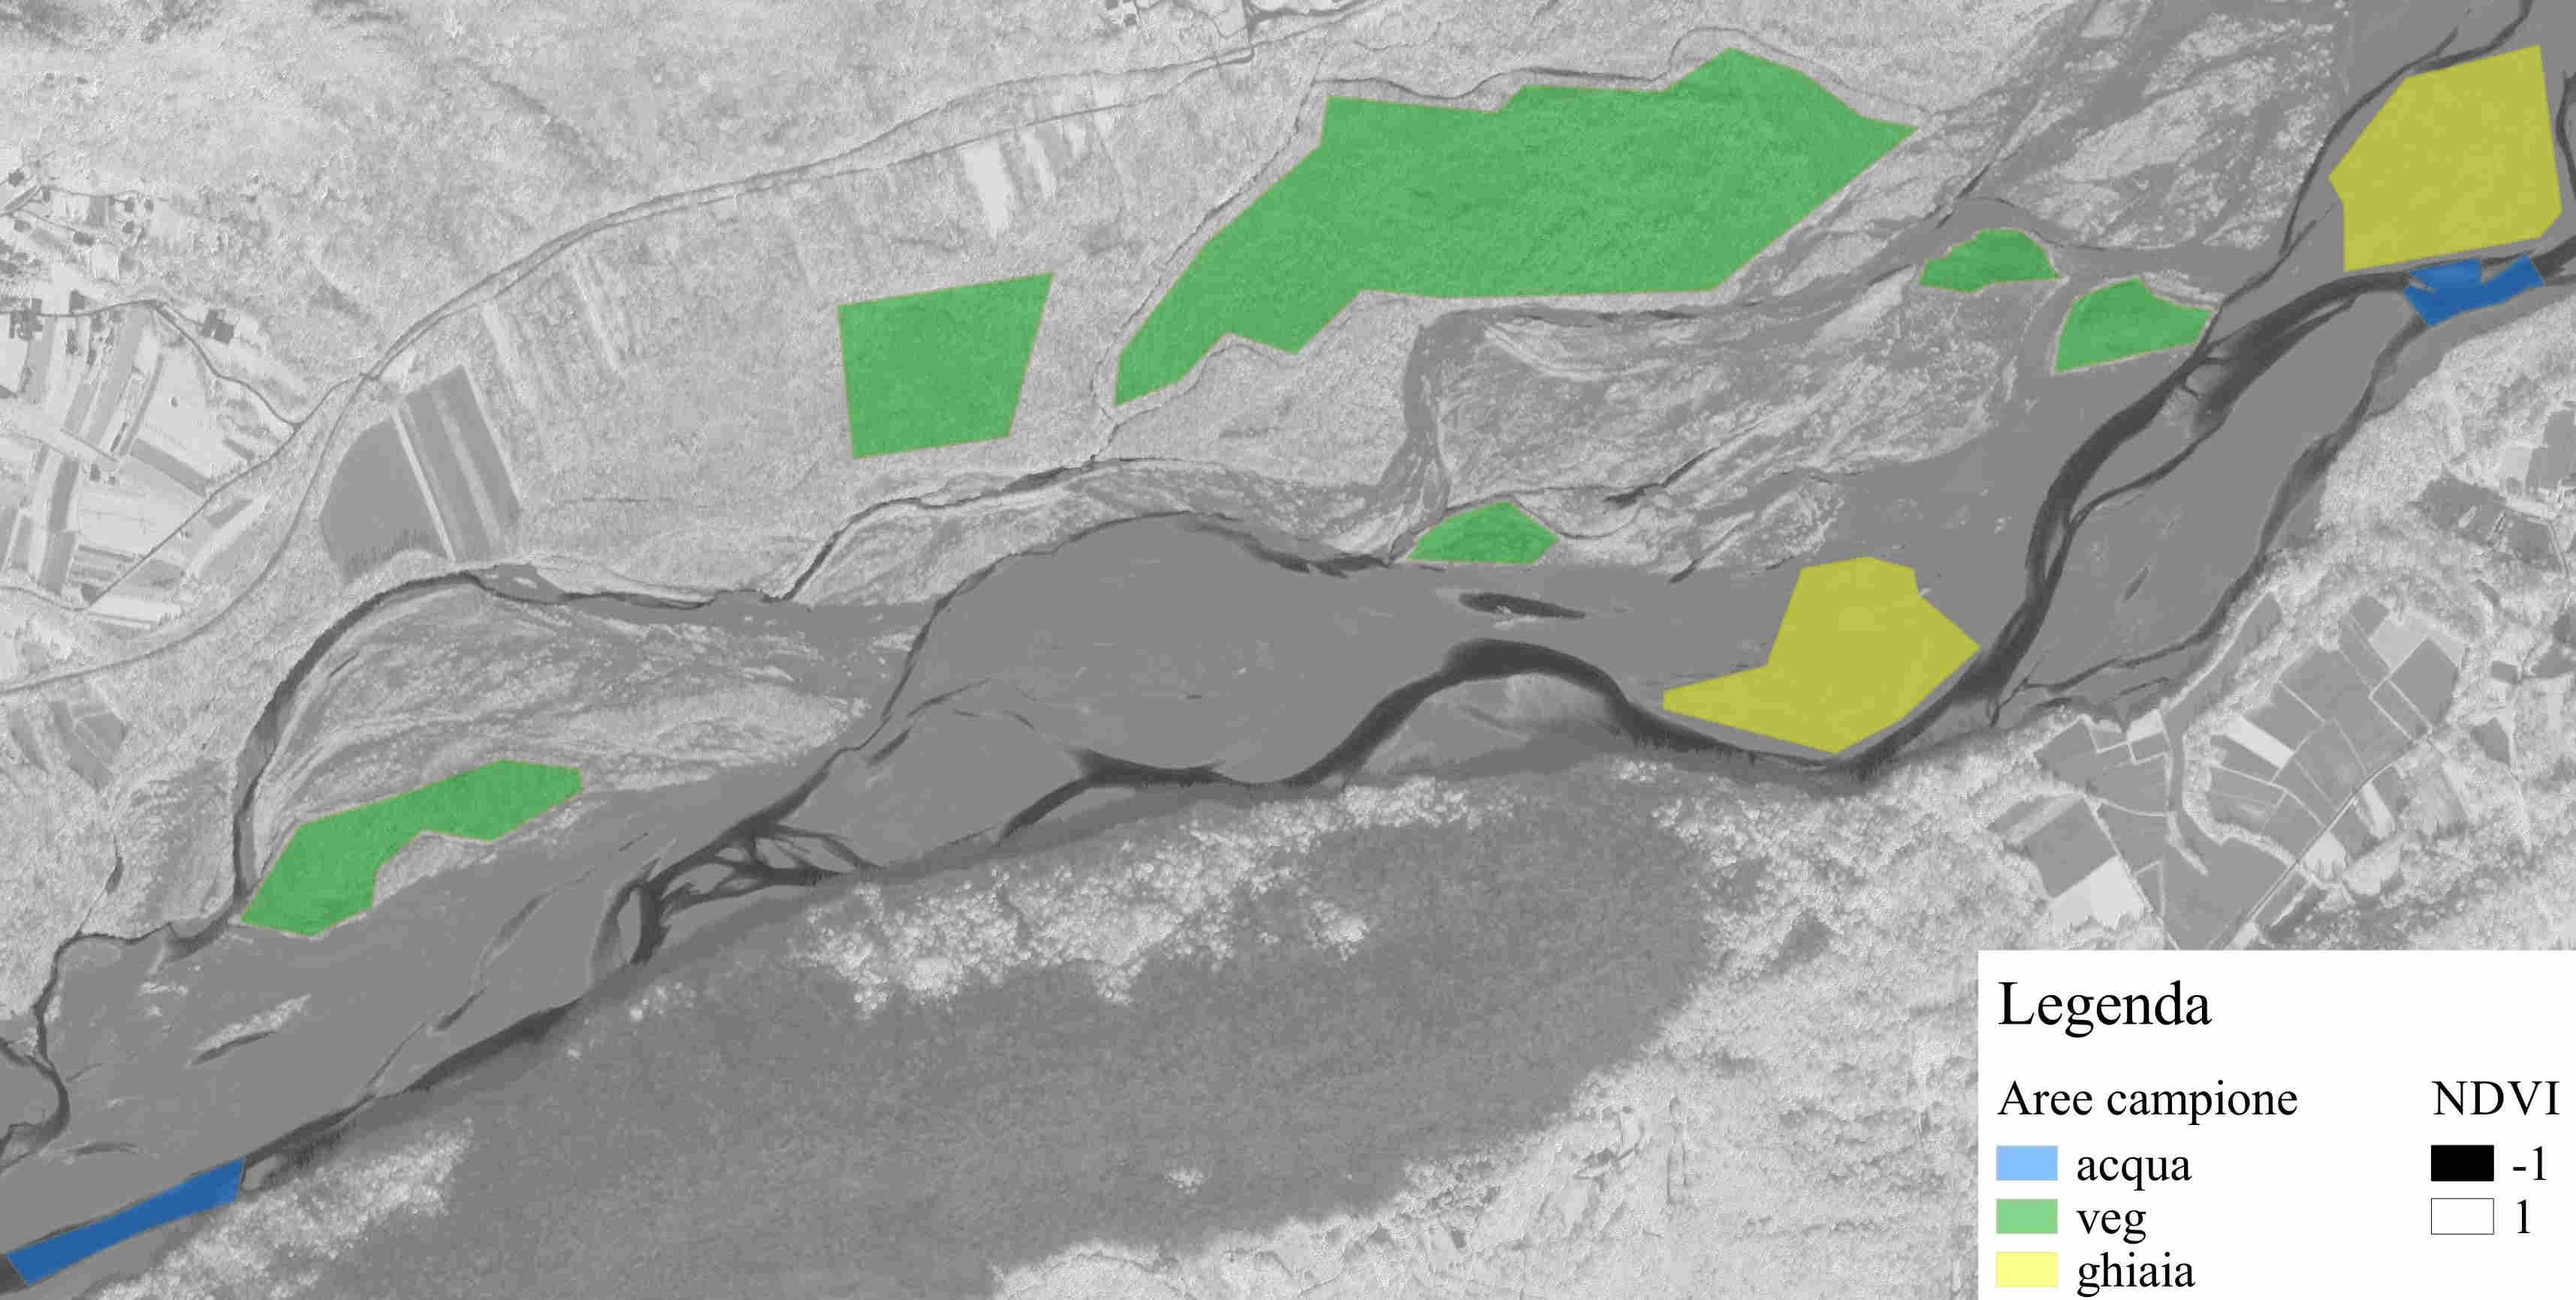
\includegraphics[width=\textwidth]{files/esempio_aree_campione_2014_10_31.jpeg}
		\caption[esempio di aree campione per calcolare la distribuzione dell'NDVI]{esempio di digitalizzazione di alcune aree campione per l'immagine \Pl{} del~2014-10-31; sullo sfondo la mappa dell'NDVI.}
		\label{fig:esempio-aree-campione}
	\end{figure}
	%
	%
	\item[Percentili aree campione]
	Per ogni immagine si è osservata la distribuzione dell'NDVI in ogni classe (\vref{graph:percentili}).
	% 
	\begin{figure}[ht]
		\centering
		\begin{tikzpicture}
	\begin{groupplot}[
		group style = {
			group size = 2 by 3,
			ylabels at = edge left,
			x descriptions at = edge bottom,
			horizontal sep = 1.1cm,
			vertical sep = 0.1cm,
		},
		width = 0.45\textwidth,
		height = 0.45\textwidth,
		ylabel = NDVI,
		boxplot/draw direction = y,
		xtick = {1,2,3},
		xticklabels = {Veg., Alveo, Canale},
		ymax = 0.795,
		ymin = -0.50,
		grid = major,
	]
	\nextgroupplot % ASTER 2005-08-31
		\addplot+ [ % vegetazione
			teal, very thick,
			boxplot prepared = {
				lower whisker = 0.353656,
				lower quartile = 0.470411,
				median = 0.560063,
				upper quartile = 0.614701,
				upper whisker = 0.644957,
				},
        	]
        	coordinates {};
		\addplot+ [ % alveo attivo
			brown, very thick,
			boxplot prepared = {
				lower whisker = 0.077472,
				lower quartile = 0.091653,
				median = 0.122488,
				upper quartile = 0.149573,
				upper whisker = 0.171459,
				},
        	]
        	coordinates {};
		\addplot+ [ % canale
			cyan, very thick,
			boxplot prepared = {
				lower whisker = -0.477885,
				lower quartile = -0.362798,
				median = -0.269905,
				upper quartile = -0.058787,
				upper whisker = 0.072414,
				},
        	]
        	coordinates {};
        \node [fill = white, draw = black, anchor = north east] 
        	at (axis description cs: 1,1) {AST 2005-08-31};
	%------------------------------------------------------
	\nextgroupplot % ASTER 2012-08-01
		\addplot+ [ % vegetazione
			teal, very thick,
			boxplot prepared = {
				lower whisker = 0.341613,
				lower quartile = 0.444200,
				median = 0.586294,
				upper quartile = 0.672889,
				upper whisker = 0.709027,
				},
        	]
        	coordinates {};
		\addplot+ [ % alveo attivo
			brown, very thick,
			boxplot prepared = {
				lower whisker = 0.10506,
				lower quartile = 0.117969,
				median = 0.143631,
				upper quartile = 0.16549,
				upper whisker = 0.184871,
				},
        	]
        	coordinates {};
		\addplot+ [ % canale
			cyan, very thick,
			boxplot prepared = {
				lower whisker = -0.432201,
				lower quartile = -0.379825,
				median = -0.322239,
				upper quartile = -0.226459,
				upper whisker = -0.103914,
				},
        	]
        	coordinates {};
        \node [fill = white, draw = black, anchor = north east] 
        	at (axis description cs: 1,1) {AST 2012-08-01};
	%------------------------------------------------------
	\nextgroupplot % Pleiades 2014-10-31
		\addplot+ [ % vegetazione
			teal, very thick,
			boxplot prepared = {
				lower whisker = 0.286467,
				lower quartile = 0.350238,
				median = 0.415502,
				upper quartile = 0.483495,
				upper whisker = 0.549505,
				},
        	]
        	coordinates {};
		\addplot+ [ % alveo attivo
			brown, very thick,
			boxplot prepared = {
				lower whisker = 0.049796,
				lower quartile = 0.055794,
				median = 0.063049,
				upper quartile = 0.07173,
				upper whisker = 0.081427,
				},
        	]
        	coordinates {};
		\addplot+ [ % canale
			cyan, very thick,
			boxplot prepared = {
				lower whisker = -0.426415,
				lower quartile = -0.387978,
				median = -0.338308,
				upper quartile = -0.266515,
				upper whisker = -0.175373,
				},
        	]
        	coordinates {};
        \node [fill = white, draw = black, anchor = north east] 
        	at (axis description cs: 1,1) {PL 2014-10-31};
	%------------------------------------------------------
	\nextgroupplot % Pleiades 2015-08-13
		\addplot+ [ % vegetazione
			teal, very thick,
			boxplot prepared = {
				lower whisker = 0.415693,
				lower quartile = 0.5,
				median = 0.570359,
				upper quartile = 0.638507,
				upper whisker = 0.704044		
,
				},
        	]
        	coordinates {};
		\addplot+ [ % alveo attivo
			brown, very thick,
			boxplot prepared = {
				lower whisker = 0.075052,
				lower quartile = 0.080858,
				median = 0.087921,
				upper quartile = 0.096031,
				upper whisker = 0.106198,
				},
        	]
        	coordinates {};
		\addplot+ [ % canale
			cyan, very thick,
			boxplot prepared = {
				lower whisker = -0.262599,
				lower quartile = -0.244228,
				median = -0.214393,
				upper quartile = -0.176471,
				upper whisker = -0.132762,
				},
        	]
        	coordinates {};
        \node [fill = white, draw = black, anchor = north east] 
        	at (axis description cs: 1,1) {PL 2015-08-13};
	%------------------------------------------------------
	\nextgroupplot % Sentinel2 2017-04-21
		\addplot+ [ % vegetazione
			teal, very thick,
			boxplot prepared = {
				lower whisker = 0.163722,
				lower quartile = 0.241916,
				median = 0.374344,
				upper quartile = 0.548241,
				upper whisker = 0.672782,
				},
        	]
        	coordinates {};
		\addplot+ [ % alveo attivo
			brown, very thick,
			boxplot prepared = {
				lower whisker = 0.056176,
				lower quartile = 0.061278,
				median = 0.067681,
				upper quartile = 0.076396,
				upper whisker = 0.089304,
				},
        	]
        	coordinates {};
		\addplot+ [ % canale
			cyan, very thick,
			boxplot prepared = {
				lower whisker = -0.322237,
				lower quartile = -0.288822,
				median = -0.239533,
				upper quartile = -0.177094,
				upper whisker = -0.131119,
				},
        	]
        	coordinates {};
        \node [fill = white, draw = black, anchor = north east] 
        	at (axis description cs: 1,1) {S2 2017-04-21};
	%------------------------------------------------------
	\nextgroupplot % WorldView2 2018-06-15
		\addplot+ [ % vegetazione
			teal, very thick,
			boxplot prepared = {
				lower whisker = 0.569665,
				lower quartile = 0.657917,
				median = 0.719523,
				upper quartile = 0.759148,
				upper whisker = 0.791594,
				},
        	]
        	coordinates {};
		\addplot+ [ % alveo attivo
			brown, very thick,
			boxplot prepared = {
				lower whisker = 0.126214,
				lower quartile = 0.129661,
				median = 0.13373,
				upper quartile = 0.138542,
				upper whisker = 0.149326,
				},
        	]
        	coordinates {};
		\addplot+ [ % canale
			cyan, very thick,
			boxplot prepared = {
				lower whisker = -0.416974,
				lower quartile = -0.392405,
				median = -0.365385,
				upper quartile = -0.335135,
				upper whisker = -0.29979,
				},
        	]
        	coordinates {};
        \node [fill = white, draw = black, anchor = north east] 
        	at (axis description cs: 1,1) {WV2 2018-06-15};
	\end{groupplot}
\end{tikzpicture}

		\caption[boxplot dell'NDVI nelle aree campione in quattro immagini satellitari]{boxplot dell'NDVI nelle aree campione in quattro immagini satellitari; i baffi indicano il 10mo e il 90mo percentile, gli estremi della scatola rappresentano il 25mo e il 75mo percentile, la linea nella scatola è la mediana.}
		\label{graph:percentili}
	\end{figure}
	%
	%
	\item[Soglie NDVI] 
	Da tali grafici sono state ottenute delle soglie di NDVI per classificare le immagini satellitari (\vref{tab:ndvi-soglia}); per l'immagine \WV{} la soglia che distingue vegetazione da alveo attivo è maggiore. Le soglie sono in accordo con quanto riportato in letteratura \squarecite{Bertoldi:2011-ASTER}.
	%
	\begin{table}[ht]
		\centering
		\begin{tabular}{
			c 
			S[table-format=1.2]@{\,}
			c@{\,}
			c@{\,}
			c@{\,}
			S[table-format=1.2]
			S[table-format=1.1]@{\,}
			c@{\,}
			c@{\,}
			c@{\,}
			S[table-format=1.1]
			}
			\toprule
			&	\multicolumn{5}{c}{\textbf{Soglie AST PL S2}}	&	\multicolumn{5}{c}{\textbf{Soglie WV2}}	\\
			\midrule
			Vegetazione		&	0.25	&	$\leq$	&	NDVI	&			&		& 	0.3	&	$\leq$	&	NDVI	&			& 	\\
			Alveo attivo	&	0.0	&	$\leq$	&	NDVI	&	$<$		&	0.25	&	0.0	&	$\leq$	&	NDVI	&	$<$		&	0.3\\
			Canale			&		&			&	NDVI	&	$<$		&	0.0	&		&			&	NDVI	&	$<$		&	0.0\\
			\bottomrule
		\end{tabular}
		\caption[soglie NDVI]{soglie di NDVI per la classificazione delle immagini satellitari.}
		\label{tab:ndvi-soglia}
	\end{table}
	%
	%
	\item[Divisione in 23 tratti]
	La maschera di calcolo è stata suddivisa manualmente in 23~tratti con 22~sezioni al fine di avere un maggior dettaglio spaziale delle dinamiche di vegetazione (\vref{fig:23-tratti}). 
	Questi tratti sono stati selezionati in modo da possedere caratteristiche omogenee per portata e crescita della vegetazione; 
	pertanto confluenze di immissari, bruschi restringimenti o allargamenti, inizio di pronunciato \emph{upwelling} o \emph{downwelling} ed evidenti cambiamenti di morfologia fluviale sono stati gli elementi per individuare le 22~sezioni che determinano i 23~tratti.
	%
	\begin{figure}
		\centering
		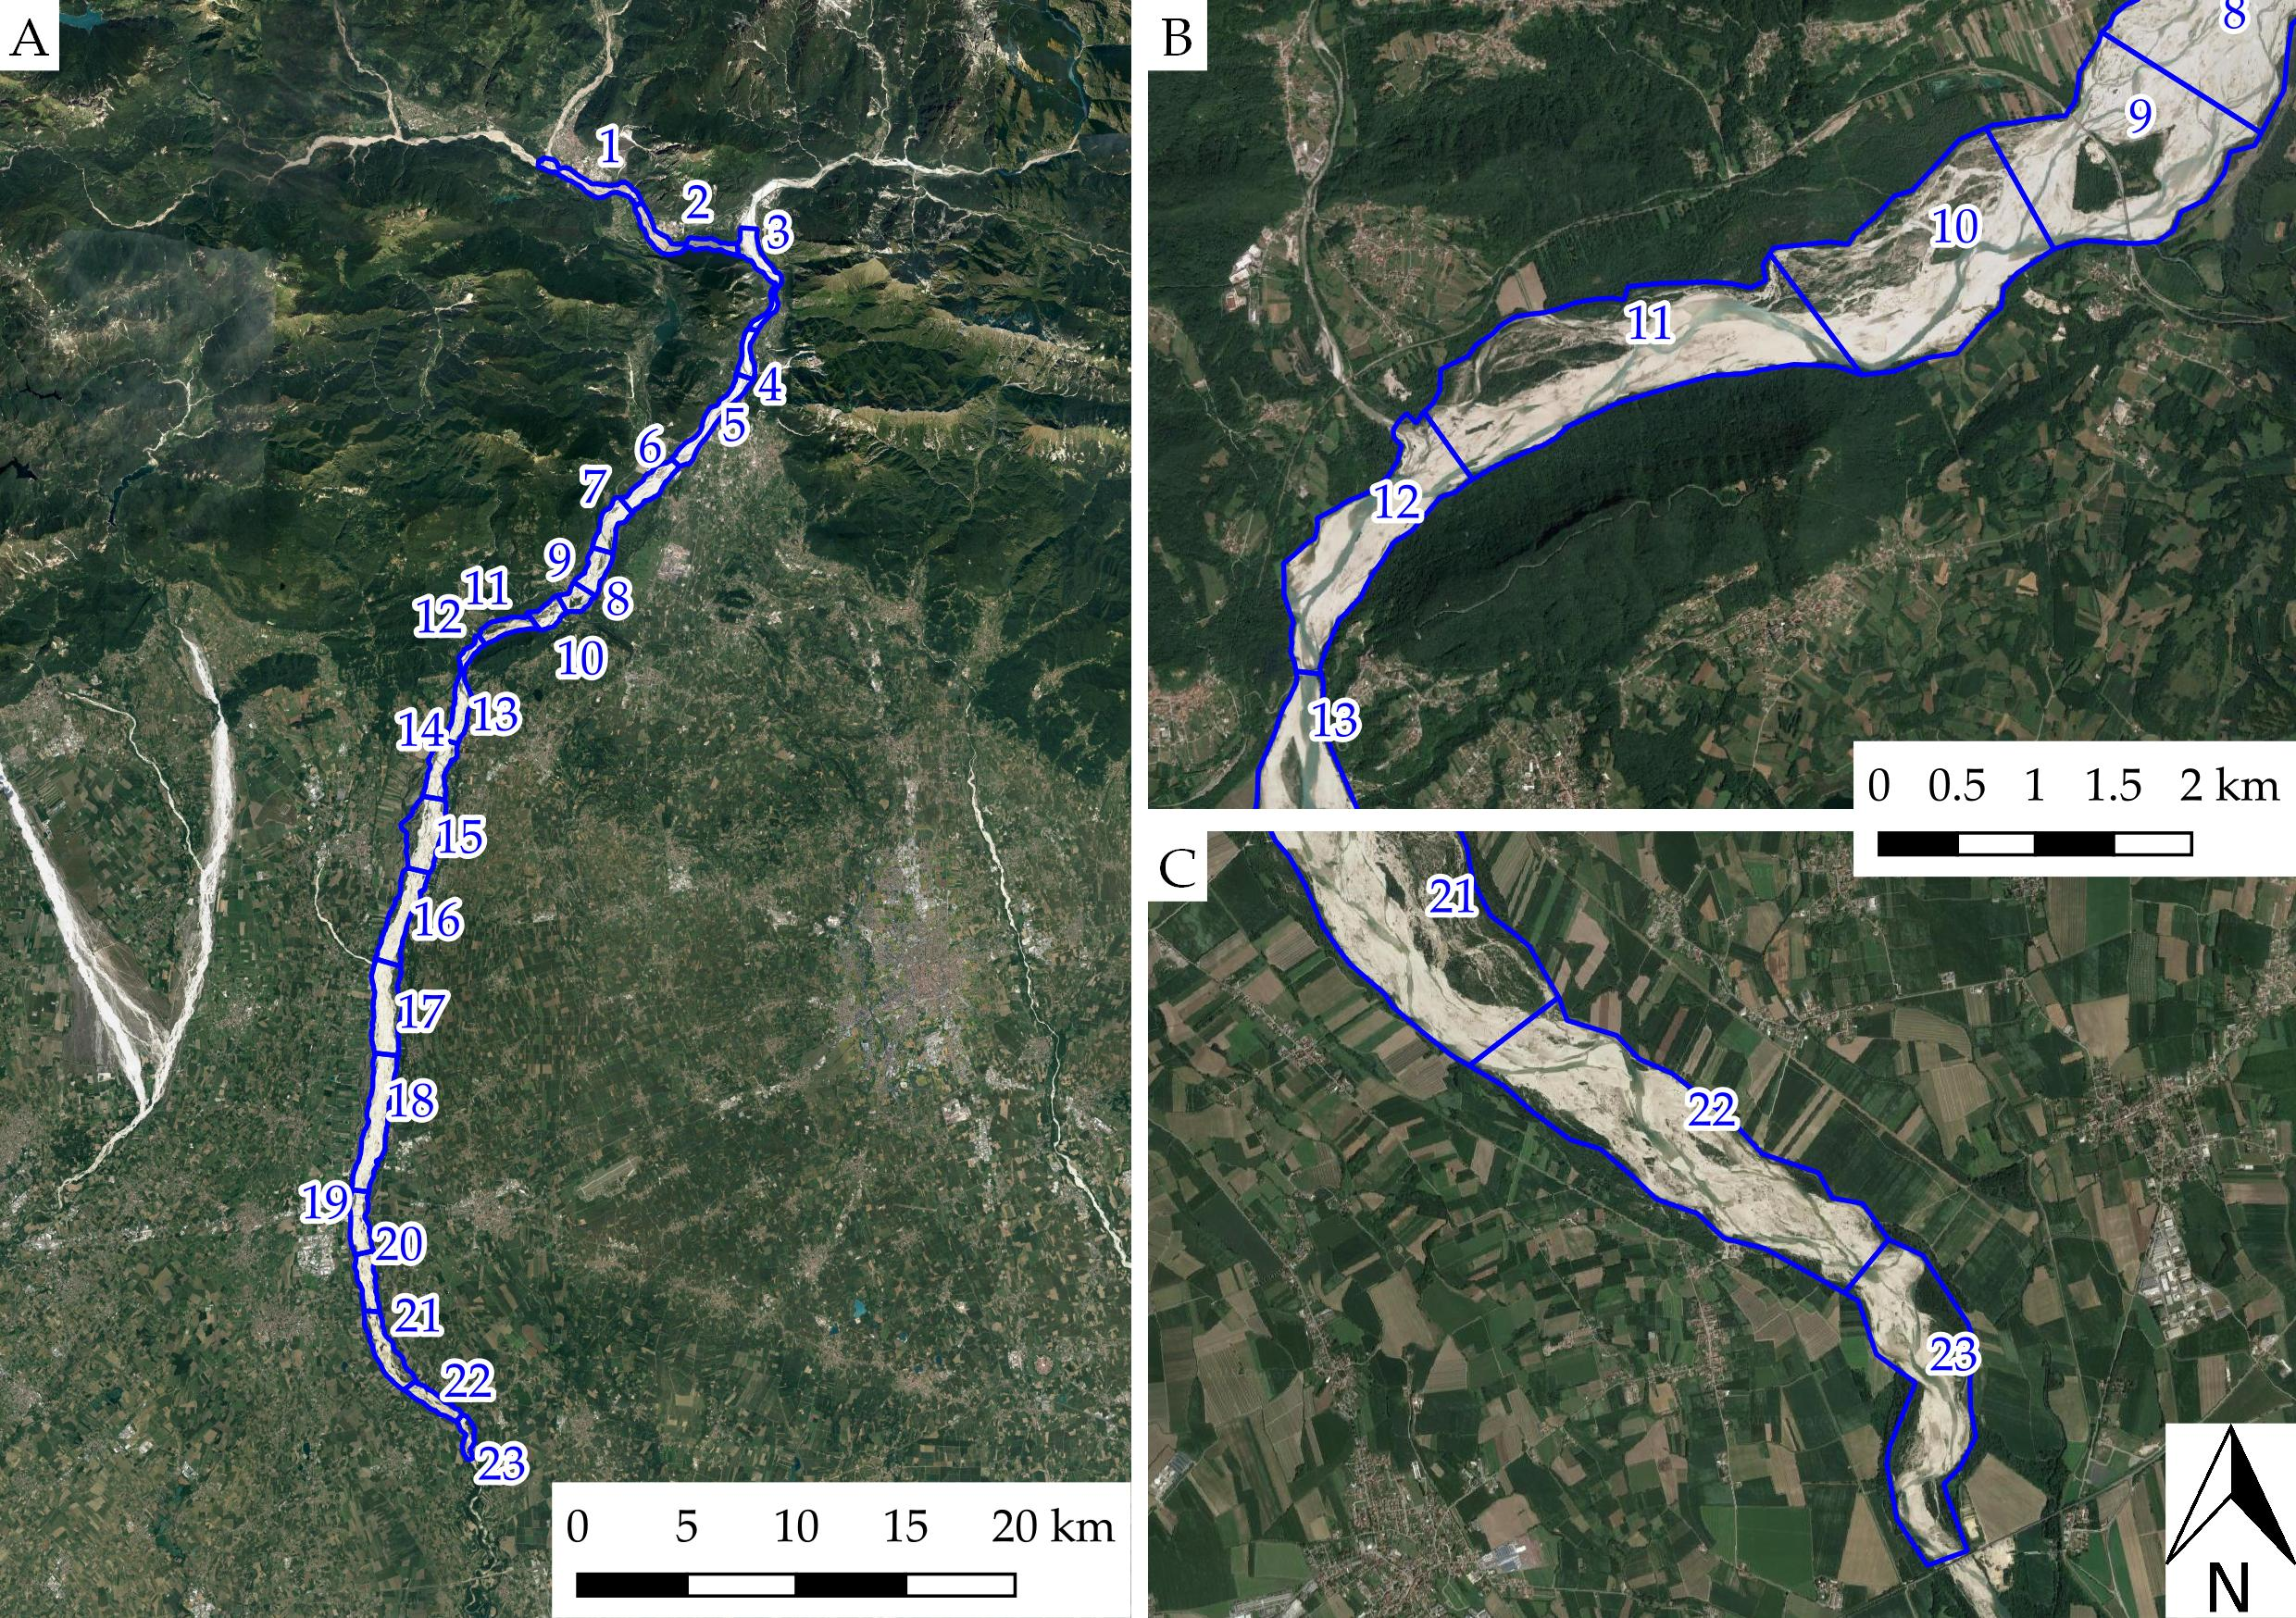
\includegraphics[width=\textwidth]{files/tutti_23_tratti.jpeg}
		\caption[immagine con la maschera suddivisa in 23 tratti]{immagine con la maschera suddivisa in 23 tratti; la sezione di monte del tratto~1 corrisponde a Tolmezzo, la sezione di valle del tratto~23 corrisponde al ponte di Madrisio.}
		\label{fig:23-tratti}
	\end{figure}
	%
	%
	\item[isole e \emph{Floodplain}]
	Tramite una procedura semi-automatica e con il supporto di Google Earth, la classe della vegetazione è stata suddivisa in \emph{floodplain} e isole. 
	Tale procedura si basa sul fatto che la maschera computazionale comprende parte della piana alluvionale e che le isole sono completamente circondate dalla ghiaia dell'alveo durante periodi di magra.
	\\
	Successivamente, un controllo visivo del risultato e una correzione manuale di alcune celle hanno permesso sia di distinguere correttamente le isole, sia di evitare che isole molto prossime alla \emph{floodplain} ne fossero considerate parte; la classe delle celle corrette è stata aggiunta alla classificazione.
	%
	%
	\item[Nuvole e nodata] Alcune immagini presentano una lieve copertura nuvolosa che si estende nella maschera; queste zone sono state manualmente delimitate poiché presentano valori NDVI alterati.
	\\
	Altre immagini hanno un'estensione limitata rispetto alla maschera; questo porta ad avere aree prive di dati (\texttt{nodata}).
	\\
	Alla classificazione sono state aggiunte la classe delle nuvole e dei \texttt{nodata}.
	%
	%
	\item[Classificazione finale dei tratti] La \vref{tab:class_tratti} mostra le classi in cui è stato classificato ognuno dei 23~tratti; la \vref{fig:class_is_fl} ne mostra un esempio.
	%
	\begin{table}[ht]
		\centering
		\begin{tabular}{
			c 
			c
			}
			\toprule
			\textbf{Macroclasse}	&	\textbf{Classe}	\\
			\midrule
			Vegetazione		&	Isola	\\
							&	Floodplain	\\
			Alveo attivo	&	Cella corretta	\\
							&	Ghiaia	\\
							&	Canale	\\
			Altro			&	Nuvola	\\
							&	Nodata	\\
			\bottomrule
		\end{tabular}
		\caption[classificazione dell'area dei tratti]{classificazione finale dell'area di ogni tratto all'interno della maschera computazionale.}
		\label{tab:class_tratti}
	\end{table}
	%
	\begin{figure}[ht]
		\centering
		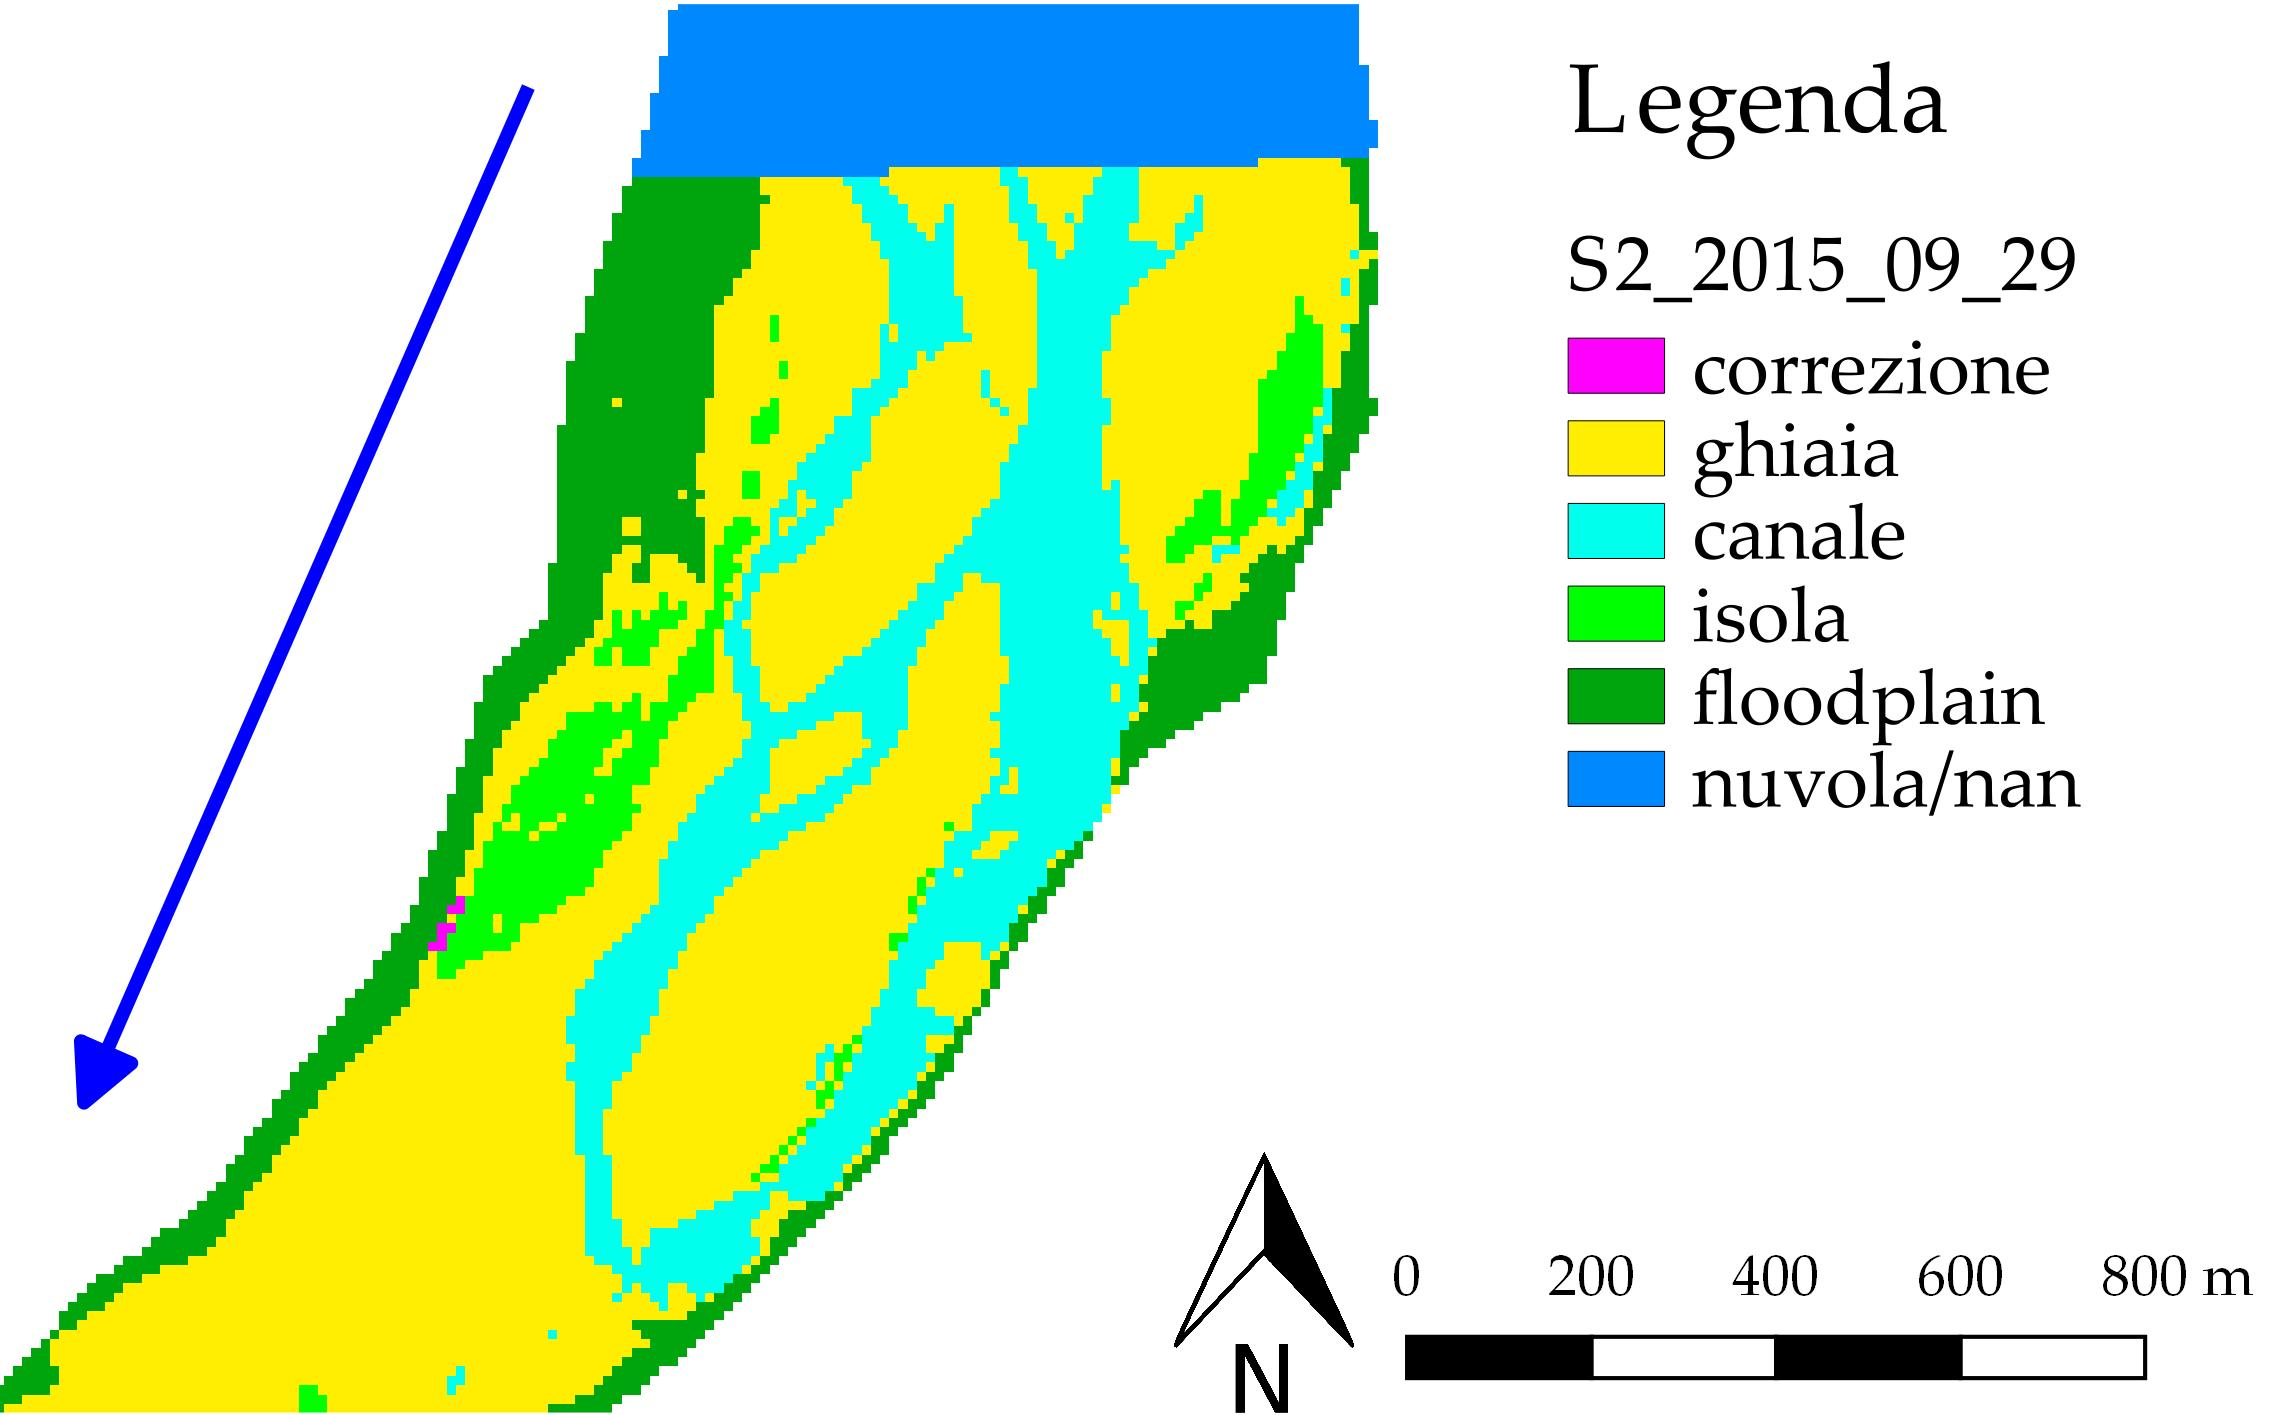
\includegraphics[width=\textwidth]{files/esempio_class_is_fl.jpeg}
		\caption[esempio della classificazione dell'area dei tratti]{esempio della classificazione dell'area dei tratti; le zone raffigurate sono rispettivamente a monte dell'isola di Cornino (in corrispondenza del monte Prat) e in corrispondenza della confluenza del Fella.}
		\label{fig:class_is_fl}
	\end{figure}
	%
Al fine di validare la precedente procedura di controllo e correzione della distinzione isole - \emph{floodplain}, si è osservato per ogni tratto l'andamento temporale della larghezza media~$B$, esprimibile semplicemente come il rapporto dell'area dell'alveo di ogni tratto (somma dell'alveo attivo e delle isole) per la sua lunghezza seguendo la corrente:
	%
	\begin{equation}
		\label{eq:larghezza-tratto}
		B = \frac{\text{Area alveo}}{Lunghezza} 
		\quad .
	\end{equation}
	% 
	Si è verificato che la larghezza~$B$ rimanesse costante nel tempo, indice di una corretta classificazione tra isole e \emph{floodplain}. 
	La~$B$ non rimane costante solo nel caso di distacco di isole o di fusione di isole nella piana. 
	\\
	La \vref{fig:b-media-7-e-15} mostra l'andamento temporale della~$B$ dei tratti~7 e~15: nel primo tratto, in cui non si osserva alcuna variazione sensibile dell'alveo, la~$B$ oscilla solo di qualche decina di metri; nel secondo si assiste alla progressiva fusione di una grande isola nella \emph{floodplain}, e questo lo si vede proprio nella diminuzione della~$B$. Ciò che conta non è quanto è largo l'alveo, ma quanto cambia la larghezza.
	%
	\begin{figure}
		\centering
		\begin{tikzpicture}
	\begin{axis}[
		width = 0.6\textwidth,
		height = 0.5\textwidth,
		date coordinates in = x,
		xticklabel = {\year},
		xticklabel style = {
			rotate = 80,
			anchor = near xticklabel
		},
		xtick distance = 730,
		enlarge x limits = 0.05,
		enlarge y limits = 0.01,
		%ymax = 3.7,
		%ymin = -0.1,
		%ytick distance = 0.5,
		ylabel = {Larghezza media dell'alveo \si{[\m]}},
		grid = major,
		]
		\addplot+
        	[blue]
        	table [x=data, y=tr_7] {graphics/data/Larghezze_medie_alveo.txt};
        \addlegendentry{Tratto 7}
        
		\addplot+
        	[orange]
        	table [x=data, y=tr_15] {graphics/data/Larghezze_medie_alveo.txt};
        \addlegendentry{Tratto 15}
	\end{axis}
\end{tikzpicture}

		\quad
		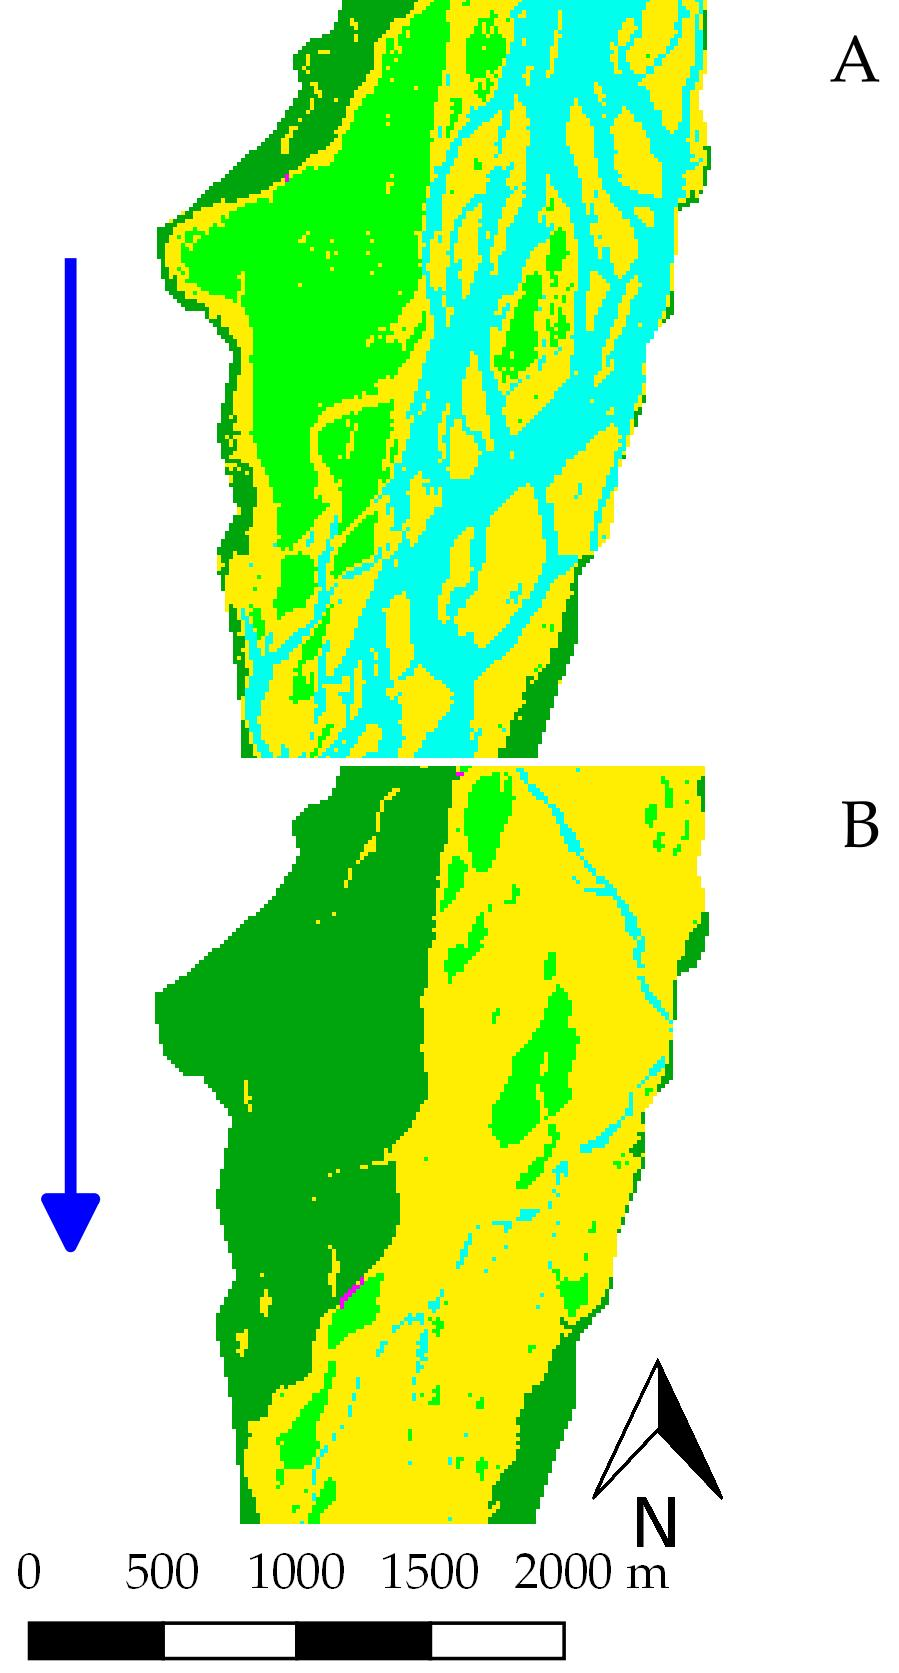
\includegraphics[width=0.3\textwidth]{files/fusione_isola_tr_15.jpeg}
		\caption[andamento temporale di $B$ per i tratti~7 e~15]{a sinistra si vede l'andamento nel tempo della larghezza media dei tratti~7 e~15; la $B$ del tratto~7 oscilla solamente di qualche decina di metri, mentre il tratto~15 riduce improvvisamente la sua $B$ a causa della fusione di una grande isola nella \emph{floodplain}, fenomeno mostrato a destra (A: 2002-06-12, B: 2005-08-30).}
		\label{fig:b-media-7-e-15}
	\end{figure}
	%
	%
	\item[Ulteriore validazione] Si è confrontata la classificazione del 2011-10-02 con la classificazione eseguita manualmente da \cite{Surian:2015} nei tratti \numrange[range-phrase={$\div$}]{6}{12} (dal ponte autostradale di Braulins alla stretta di Pinzano).
	Le mappe di classificazione del 2005-08-30, 2010-09-29, 2013-09-05 sono state confrontate con i CSM ricavati dai rilievi aerei LiDAR eseguiti nei corrispondenti anni sui tratti \numrange[range-phrase={$\div$}]{6}{12} (\vref{fig:validazione-class-is-fl}).
	%	
	\begin{figure}
		\centering
		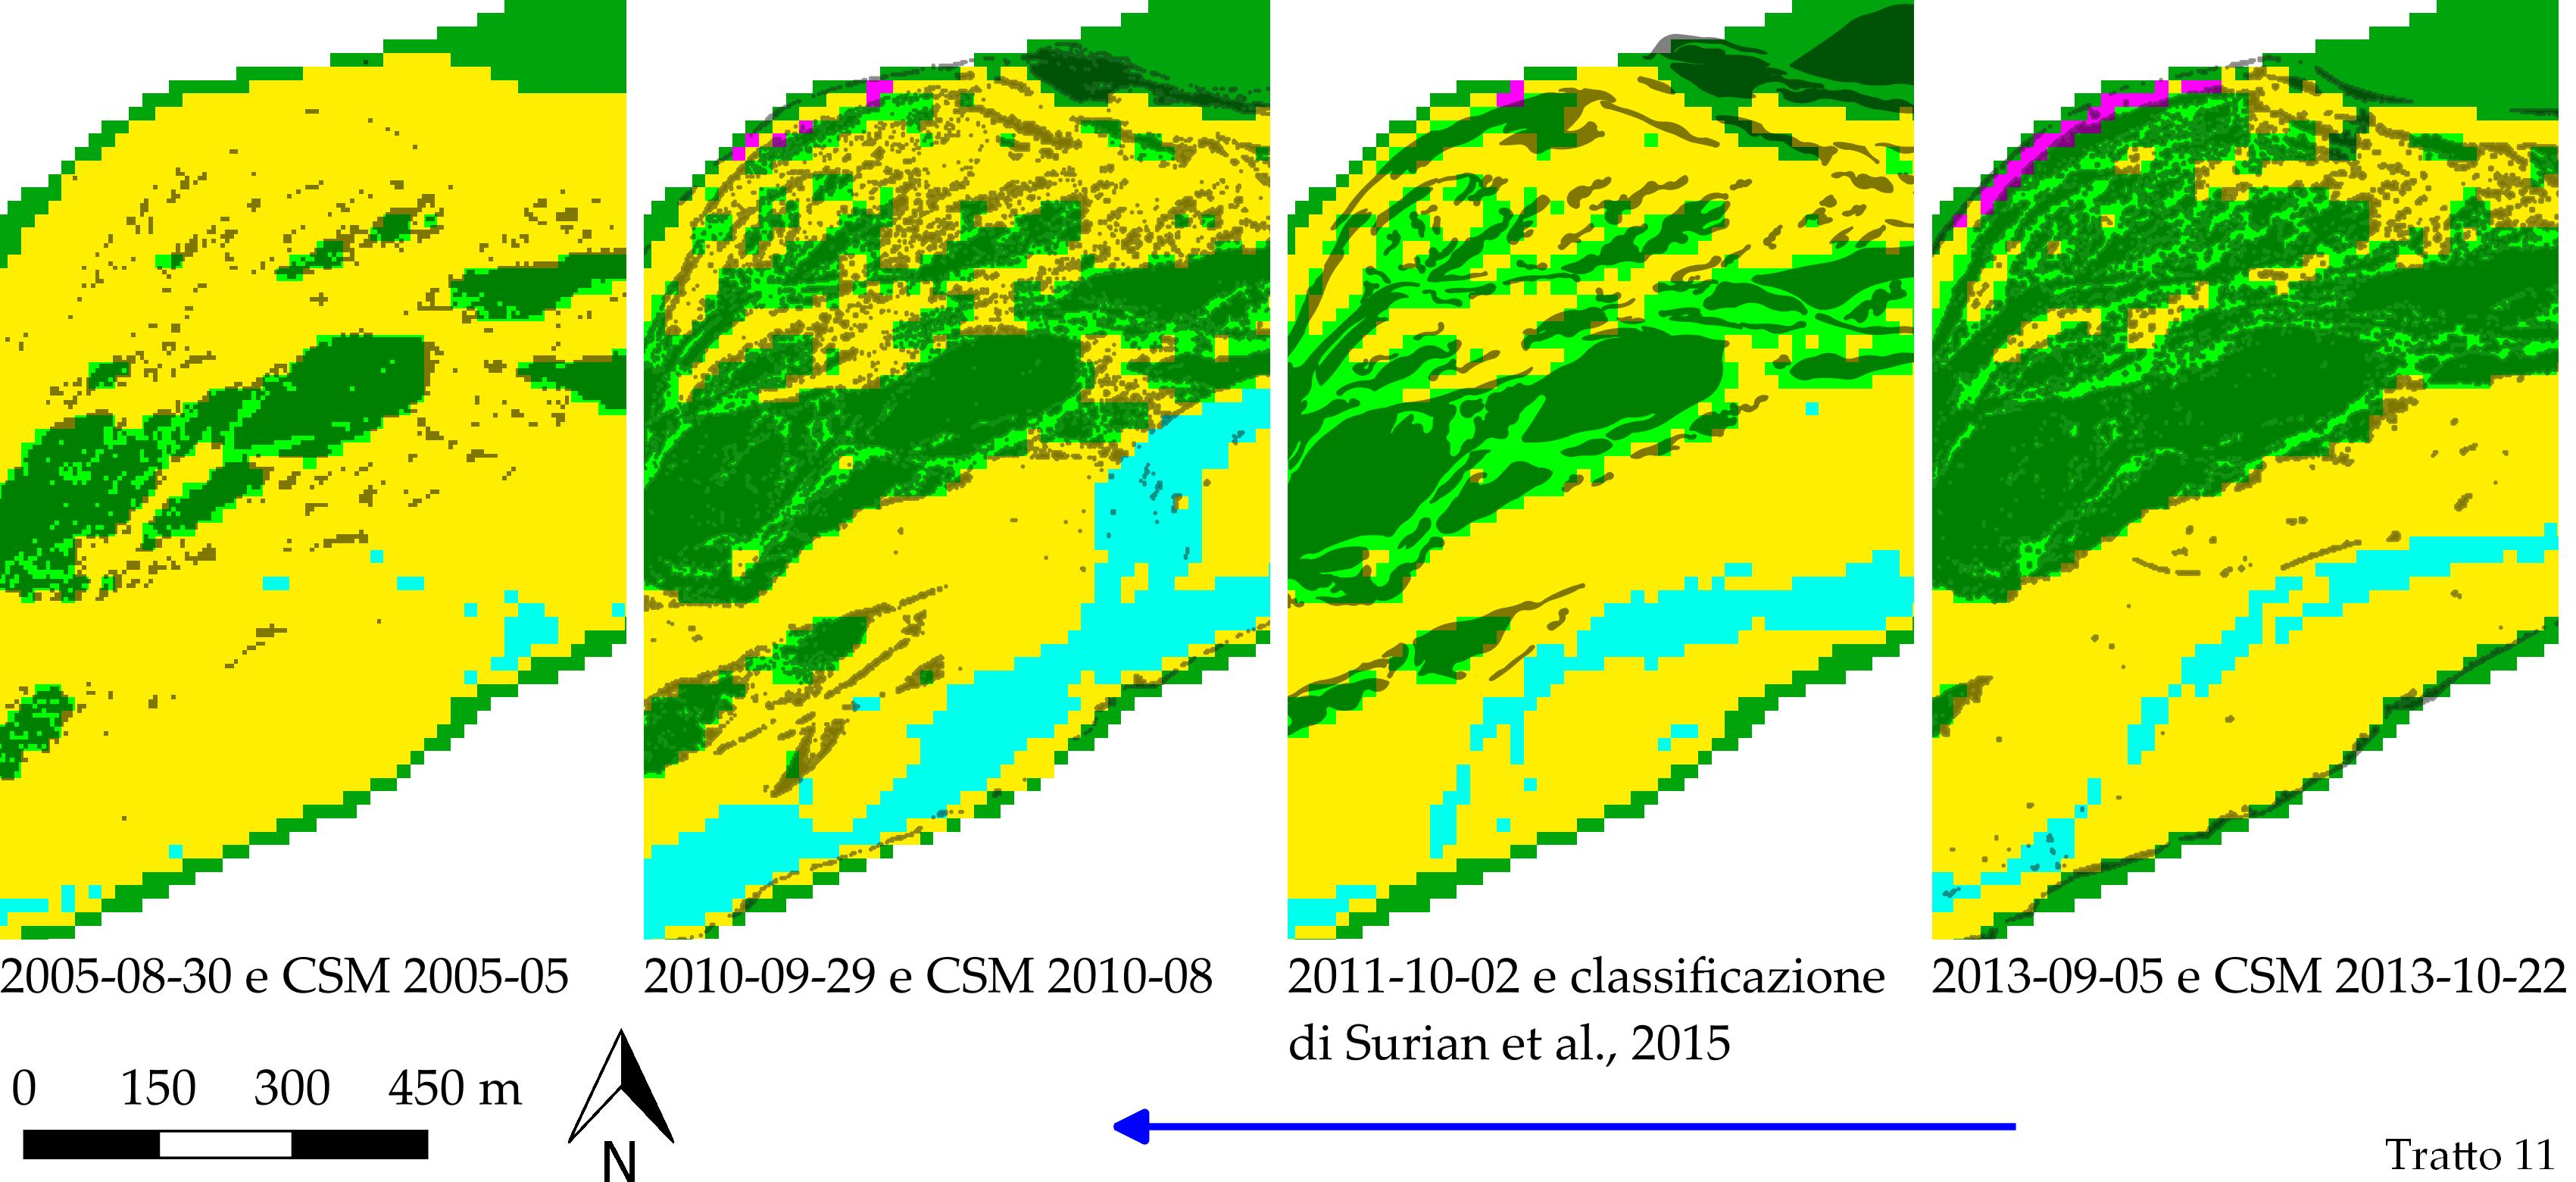
\includegraphics[width=\textwidth]{files/Class_mia_vs_surian_csm.jpeg}
		\caption[validazione della classificazione dell'alveo]{confronto tra le mappe di classificazione dell'alveo e i CSM dai rilievi aerei LiDAR e la classificazione manuale eseguita in \cite{Surian:2015}; le aree scure corrispondono alla vegetazione individuata nei CSM e dalla classificazione manuale; per la legenda delle mappe di classificazione dell'alveo vedere la \vref{fig:class_is_fl}.}
		\label{fig:validazione-class-is-fl}
	\end{figure}
	%
	\\
	Visualmente si verifiche che c'è sostanziale corrispondenza tra le classificazioni ottenute dalle immagini satellitari e la vegetazione individuata dai CSM, così come tra la classificazione manuale di \cite{Surian:2015} e la mappa del 2011-10-22.
	\\
	Esiste una certa differenza tra la classificazione manuale e quella semi-automatica utilizzata nel presente lavoro: la metodologia con cui si procede influisce sul risultato finale.
	Avendo \cite{Surian:2015} utilizzato ortofoto ad alta risoluzione (\SI{0.1}{\m}), hanno potuto facilmente distinguere le chiome dei singoli alberi dalla ghiaia o vegetazione bassa circostante; le immagini satellitari utilizzate (principalmente a risoluzione di \SI{10}{\m} o \SI{15}{\m}) permettono invece di osservare macchie di vegetazione.
	In quanto si considera come isola non solo la vegetazione presente all'interno dell'alveo attivo, ma anche la zona meno vegetata posta circa alla medesima quota, l'approccio seguito sembra delineare più nettamente il contorno delle isole maggiori, sebbene le isole più piccole (con estensione minore di una cella) non siano individuate.
	\\
	Un rapido confronto delle mappe di classificazione \Pl{} e \WV{} ad alta risoluzione (\SI{0.5}{\m}) con le mappe di classificazione manuale e il CSM del 2013-10-22 mostra una sovrapposizione quasi completa della vegetazione individuata con i diversi metodi.
	\\
	A fronte di quanto esposto, si ritiene che la classificazione eseguita sia sufficientemente validata.
\end{description}


\begin{comment}
%TODO tenere questa parte? forse la si può togliere
% e mostrare direttamente i risultati sul cambiamento
Con la riclassificazione delle immagini dell'NDVI rispetto alle soglie proposte è stato possibile ottenere la percentuale di alveo coperta da vegetazione per ogni anno. 
Si ricorda, grazie alla maschera applicata, tale copertura include sia isole vegetate sia la parte di piana alluvionale che nel periodo di studio ha esperito fenomeni di erosione della vegetazione e quindi espansione dell'alveo attivo.
Infine, per le immagini l'alveo parzialmente coperto da nuvole, la maschera è stata estesa per escludere tali zone coperte poiché queste presentano valori di NDVI non corretti.
\\
I risultati sono mostrati nel grafico in \vref{graph:class-sat-veg}.


\begin{figure}[ht]
	\centering
	\begin{tikzpicture}
	\begin{axis}[
		width = \textwidth,
		height = 0.5\textwidth,
		date coordinates in = x,
		date ZERO = 2000-01-01,
		xticklabel = {\year},
		xticklabel style = {
			rotate = 80,
			anchor = near xticklabel
		},
		axis y line* = right,
		ymax = 70,
		%ymin = 0,
		ylabel = {Percentuale di vegetazione},
		grid = none,
		]
		\addplot+
        	[red, mark=+, ultra thick]
        	table [x=data, y=veg] {graphics/data/Class_sat_veg-H2O-ghiaia.txt};
	\end{axis}
	
	\begin{axis}[
		width = \textwidth,
		height = 0.5\textwidth,
		date coordinates in = x,
		date ZERO = 2000-01-01,
		xticklabel = {\year},
		xticklabel style = {
			rotate = 80,
			anchor = near xticklabel
		},
		axis y line* = left,
		axis x line = none,
		enlarge x limits = 0.05,
		enlarge y limits = 0.01,
		ymax = 3.7,
		ymin = 2,
		ylabel = {Livello idrometrico},
		grid = none,
		]
		\addplot+
        	[blue, no markers, ultra thin]
        	table [x=data, y=media-gg] {graphics/data/Dati_Villuzza.csv};
	\end{axis}
\end{tikzpicture}

	\caption[andamento dell'areale della vegetazione nelle isole  e nella floodplain]{andamento dell'areale della vegetazione nelle isole e nella floodplain (in rosso). I dati provengono dalla classificazione delle immagini satellitari (\AST{}, \Pl{}, \Se{} e \WV{}). In blu sono mostrati i livelli idrometrici medi giornalieri superiori a~\SI{2}{\m} registrati alla stazione di Villuzza.}
	\label{graph:class-sat-veg}
\end{figure}
% grafico piene 2m+ - %veg tratti (nuovo file comprensivo di tutti i tratti)
\end{comment}



\subsection{Risultati: evoluzione della larghezza}
Utilizzando le mappe di classificazione del terreno all'interno della maschera computazionale, si è ottenuta una larghezza media~$B$ secondo l'equazione~\eqref{eq:larghezza-tratto}.
%TODO \vref{eq:larghezza-tratto}. 
\\
Osservando la variazione temporale di~$B$ è possibile evincere delle traiettorie evolutive sia a livello di singolo tratto, sia a scala più ampia.
Inoltre, considerando la variazione spaziale (da monte verso valle) dell'areale delle isole, sono evidenti i pattern di \emph{upwelling} o \emph{downwelling} utilizzati durante la definizione dei 23~tratti.

